\documentclass[chapter, oneside]{oblivoir}
\usepackage{kotex}
\usepackage{graphicx}
\usepackage{mathtools}
\usepackage{hyperref} 
\hypersetup{colorlinks=false,}  
\usepackage{fapapersize}
\usefapapersize{210mm, 297mm,30mm,*,35mm,30mm}
\title{Where \TeX?}
\author{esctabcapslock}
\makeindex

\begin{document}
\maketitle
%\tableofcontents

\begin{abstract}
    이제까지 \LaTeX에 대해 알아 봤다면, 이번에는 직접 \LaTeX을 만져 볼 시간이다. 막막하다. 어디서 깔아야 하는 거지? 이 `Where'의 질문에 대답해 주겠다. \LaTeX를 사용하는 방법에는 크게 2가지가 있다. overleaf를 이용해서 웹 상에서 \LaTeX을 이용하는 방법과, 컴퓨터에 직접 \LaTeX을 까는 방법이다. 이제부터 이 들 방법에 대해 알아 볼 것이다.
\end{abstract}

\section{설치 없이 사용하기}
무언가를 컴퓨터에 설치한다는 일은 버겁고 귀찮은 일이라고 할 수 있다. 설치할 때 이것 저것 신경 써야 하고, 또 컴퓨터의 용량을 차지하게 된다. overleaf를 사용하면 이러한 문제를 해결할 수 있다.

\subsection{overleaf란?}
\begin{figure}[h!]
\centering
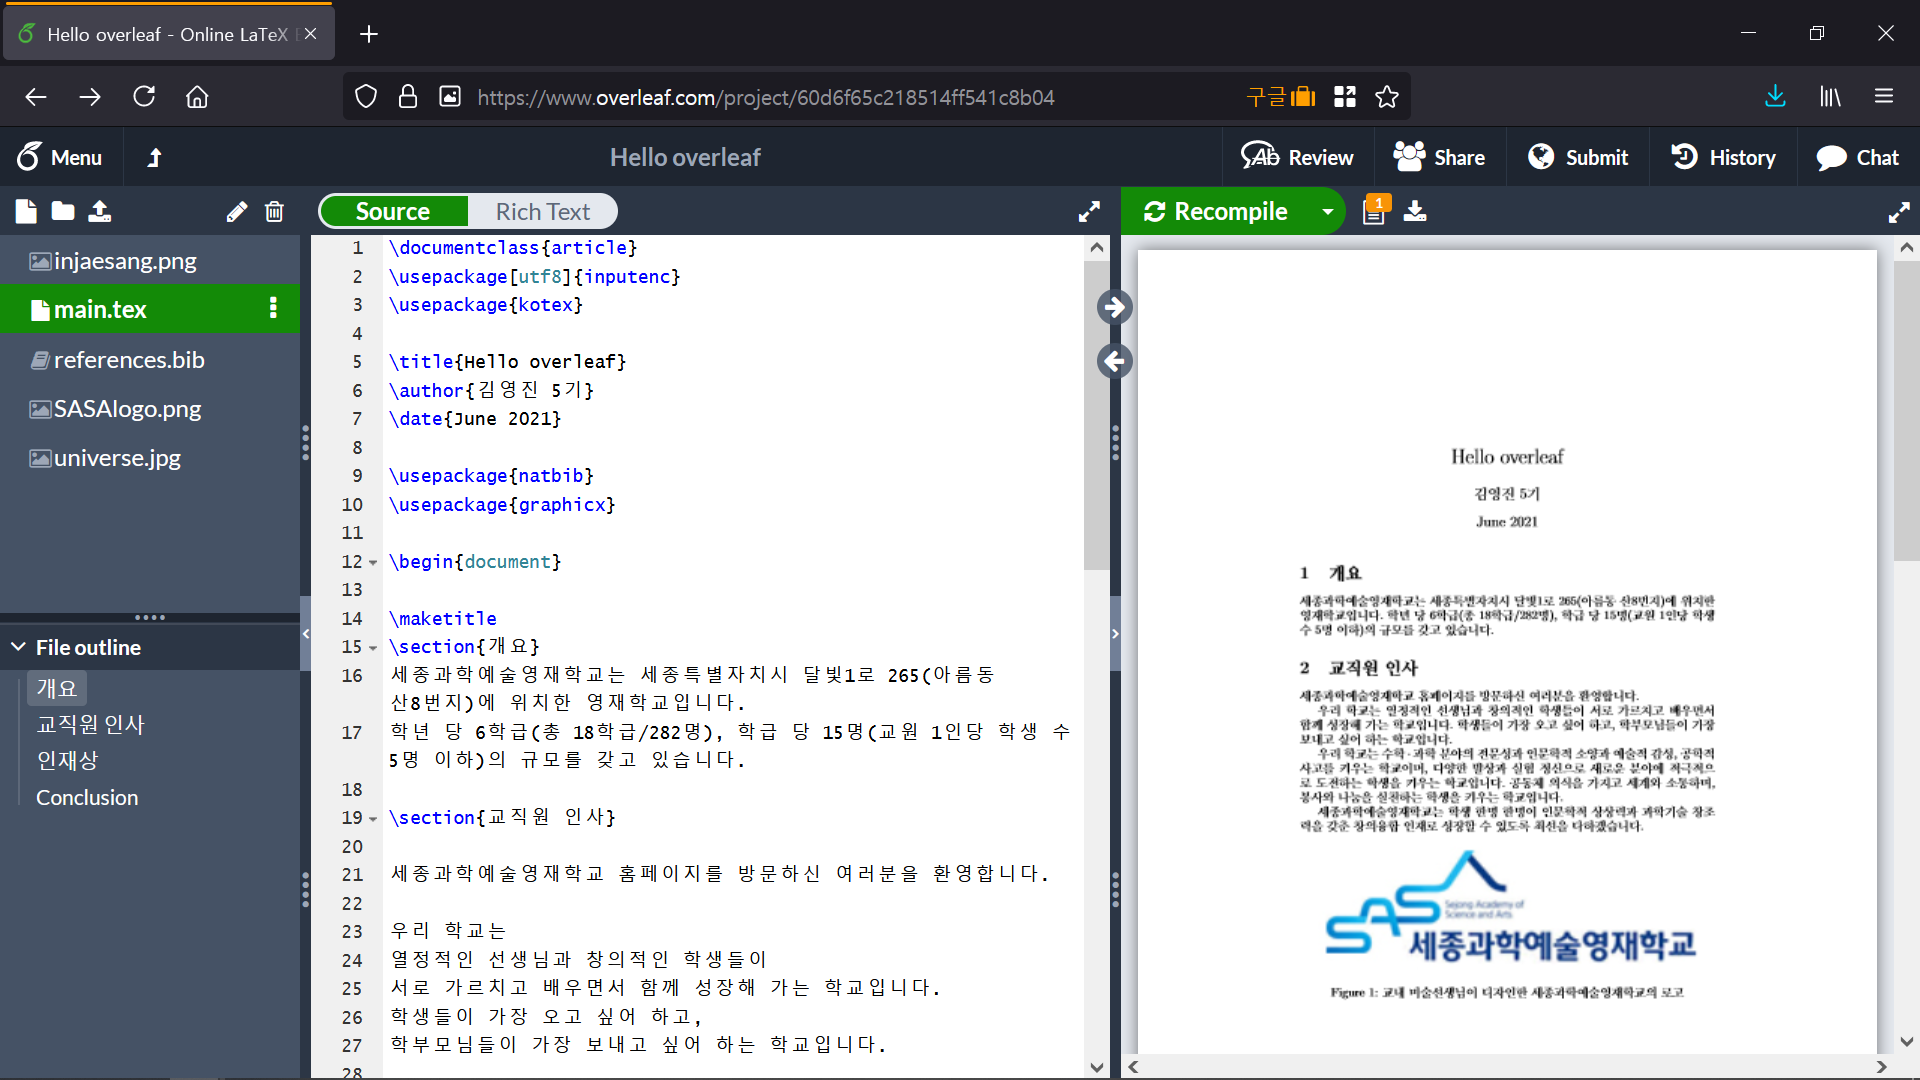
\includegraphics[width=.7\textwidth]{img/5/overleaf.edit.png}
\caption{overleaf의 편집 화면}
\label{overleaf:edit}
\end{figure}

overleaf란 온라인 \LaTeX 에디터이다. 구글 독스를 생각하면 얼추 비슷하다. 온라인에서 문서를 편집할 수 있고, 또, 다른 사람들과 협업도 가능하다. overleaf도 마찬가지의 기능을 제공한다. 컴파일도 해준다. 심지어 WYSIWYG 기능도 있어 마치, 한글 문서를 작성하는 것 처럼 \LaTeX 문서를 작성할 수 있다.

\subsection{장점}

\subsection{overleaf란?}
\begin{figure}[h!]
\centering
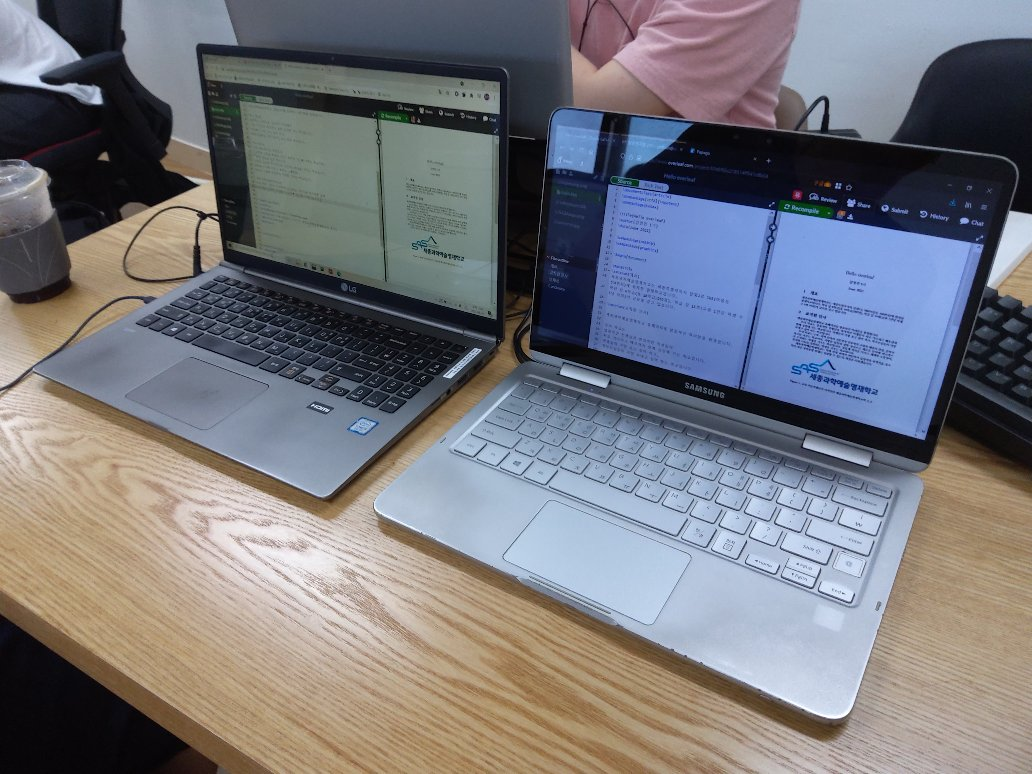
\includegraphics[width=.7\textwidth]{img/5/overleaf_shere.jpg}
\caption{overleaf의 공동 작업 기능을 이용하는 모습}
\label{overleaf:shere}
\end{figure}

\begin{itemize}
\item  어느 기기에서나 쉽게 \LaTeX을 편집할 수 있다.
\item  영어 맞춤법 검사 기능이 있다.
\item  코드 자동완성 기능이 있다.
\item  대부분의 패키지가 설치되어 있다.
\item  간단한 WYSIWYG\footnote{What You See Is What You Get, ``보는 대로 얻는다''라는 뜻으로 문서 편집 과정에서 화면에 포맷된 낱말, 문장이 출력물과 동일하게 나오는 방식을 말한다. 한글, MS워드 등 대부분의 워드 프로세서가 체택한 방식이다. 반면 HTML, 마크다운, \Tex등은 편집 명령어를 통해 편집하므로 이와 구분된다.}
기능을 제공한다. 우측 상단의 `Rich Text'버튼을 누르면, 한글 문서를 작성하듯이 \LaTeX 문서를 작성할 수 있다.
\item 쉽게 내 문서를 공유할 수 있다.
\item  공동 작업이 쉽다. 우측 상단에 `Share'버튼을 클릭하면 된다. 공동 작업에 필요한 여러 부가 기능도 제공하니 잘 활용해 보자.
\end{itemize}


\subsection{단점}
\begin{itemize}
    \item  인터넷이 있어야만 이용할 수 있다.
    \item  회원가입을 해야 사이트를 이용할 수 있다.
    \item  무료 사용자의 기능을 제한한다. 다만 무료 버전도 개인이  큰 무리 없이 사용 가능하다.
    \item 사이트가 영어로만 되어 있다.
\end{itemize}


\subsection{overleaf 시작하기}
\begin{enumerate}

\begin{figure}[h!]
\centering
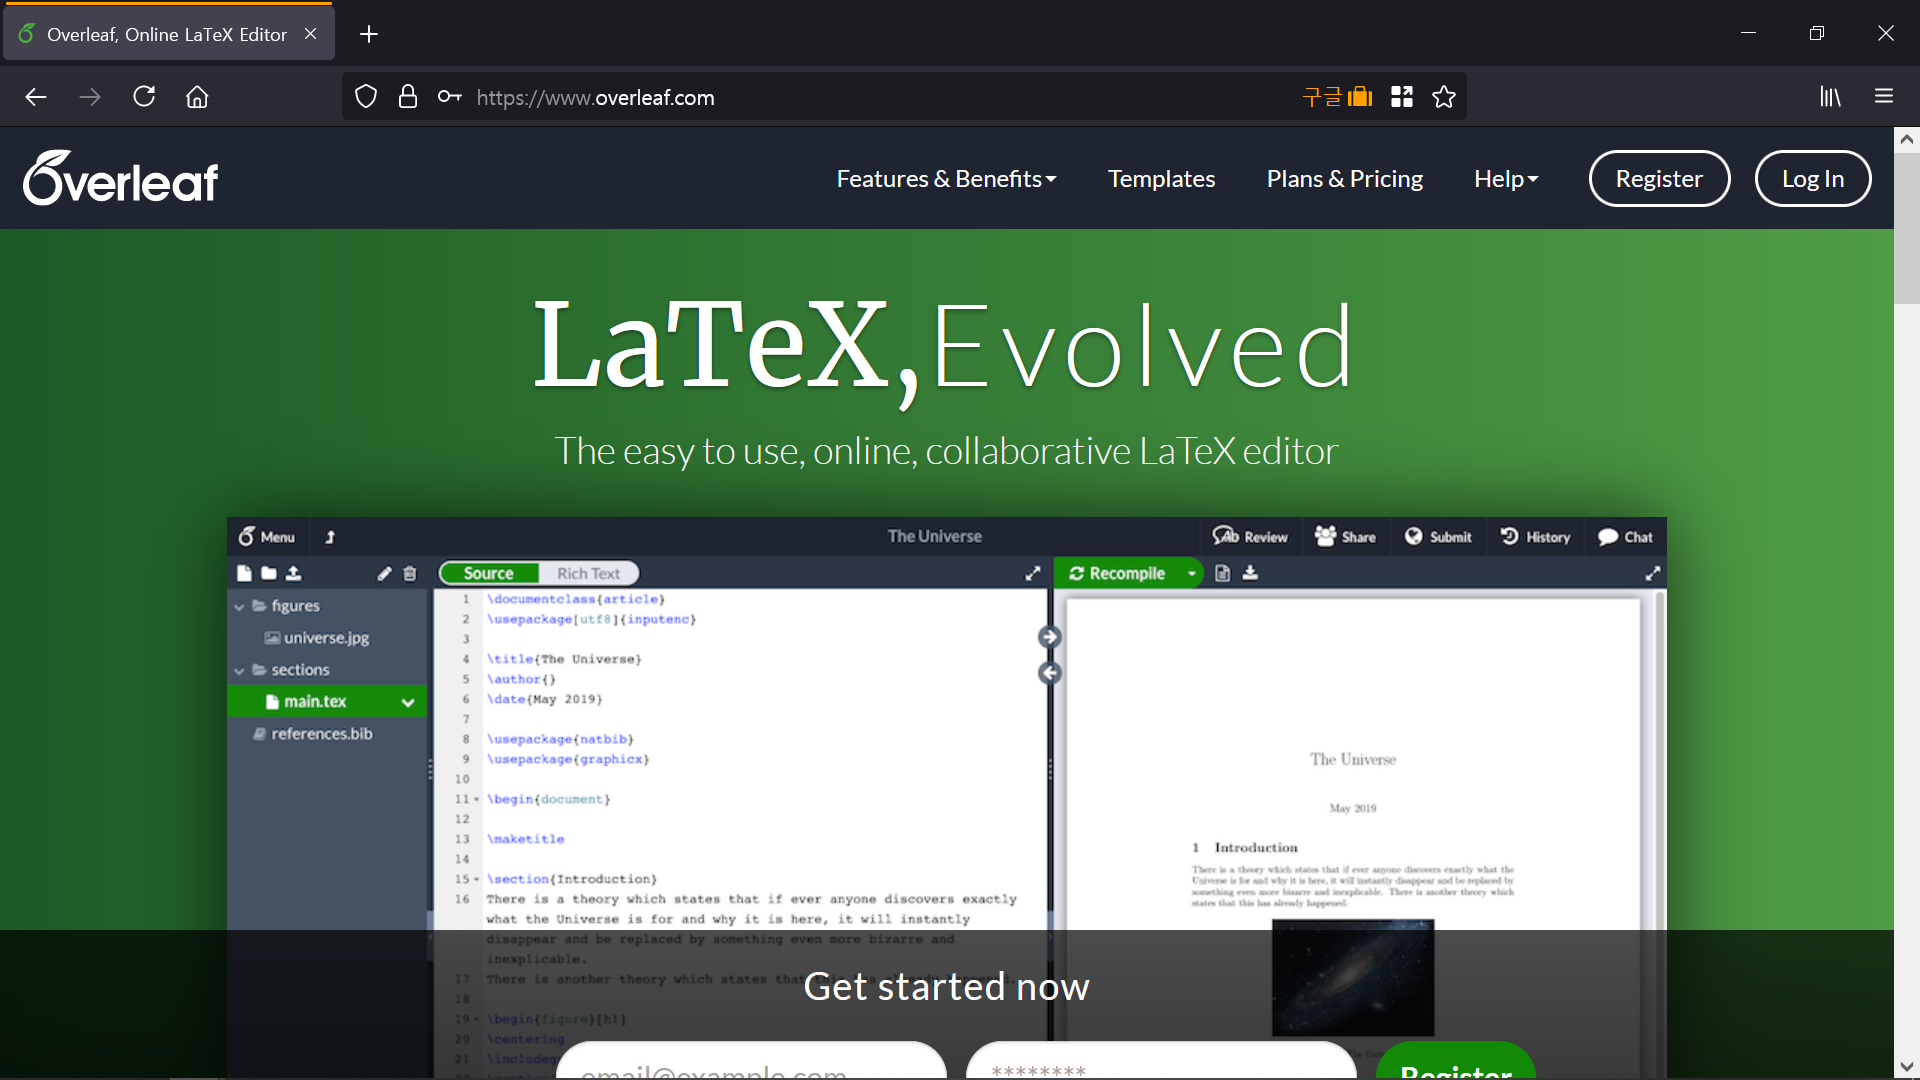
\includegraphics[width=.7\textwidth]{img/5/overleaf_main.png}
\caption{overleaf에 처음 접속했을 때 보이는 화면}
\label{overleaf:main}
\end{figure}
\item  www.overleaf.com에 접속한다.
\item  오른쪽 상단의 ``Register''버튼을 눌러 회원가입한다.
\item  이메일 주소를 이용해 회원가입을 하거나, 구글 계정을 통해 가입할 수 있다. 세종과학예술영재학교 가족이라면, 구글 계정 기반의 학교 계정을 통해 손쉽게 가입할 수 있다.
\item  ``Welcome to Overleaf''라는 문구가 당신을 반겨 줄 것이다. ``Create First Project''를 눌러 새로운 \LaTeX 프로젝트를 생성하자. 우리는 초보자니까 ``Example Project''를 클릭하도록 하자
\item  새로운 프로젝트의 이름을 입력하라는 창이 뜬다. 적당히 잘 짓는다.
\item  이제 모든 준비가 끝났다. 즐길 시간이다!
\item  적당히 글을 썼다면, 컴파일을 해야 글이 보인다. 컴파일은 단축기 Ctrl+S, Ctrl+Enter를 이용하거나, 중앙 상단의 `Recompile'버튼을 누르면 된다.
\item  만약, 사진 등 다른 파일을 \TeX 문서에 삽입하고 싶다면, 왼쪽 상단의 업로드 버튼을 클릭해서 파일을 업로드해야 한다.
\end{enumerate}

\section{내 컴퓨터에 설치하기}
overleaf는 인터넷이 있어야만 사용할 수 있다는 엄청난 단점을 갖고 있다. \LaTeX을 맛 보는 데는 overleaf도 좋지만, \LaTeX의 심연의 맛을 느끼고 싶다면, 컴퓨터에 직접 \LaTeX을 깔아야 한다. \TeX은 단지 조판 프로그렘일 뿐이므로, 도널드 커누스(Donald Ervin Knuth)가 만든 그 \TeX만으로는 무언가를 하기 매우 힘들다. 따라서, 우리는 \TeX과 관련 패키지들을 묶어 놓은 \LaTeX를 이용해야 한다. 그리고 이를 사용하기 위해 \TeX배포판을 다운받을 것이다. \TeX배포판중 가장 유명한 것이 TeXLive라는 프로그램이다.
\subsection{장점}
\begin{itemize}
    \item 오프라인에서 사용 가능하다.
    \item 커스터마이징의 자유도가 높다.
    \item 입맛에 맞는 에디터를 사용할 수 있다.
\end{itemize}

\subsection{단점}
\begin{itemize}
    \item 설치가 오래걸린다.
    \item 프로그렘의 용량이 큰 편이다. (몇 기가)
\end{itemize}


\subsection{TeXLive 설치}
TeXLive는 Windows, macOS, Linux 운영체제에 설치할 수 있다. 이 문서에서는, 가장 대중적(?)인 운영체제인 Windows에서의 설치를 다룰 것이다. 다른 OS의 경우, `http://wiki.ktug.org/wiki/wiki.php/설치'를 참조하여라. 본 글도 위 사이트를 참조한 것이다. (한국 \TeX 사용자 협회)

\paragraph{설치 전 주의사항}
TeXLive설치에는 마음에 준비가 필요하다. 실행 파일(.exe)을 이용한 TeXLive의 설치는 서너시간이 소요된다. 따라서 안정적인 인터넷 연결과 충분한 시간, 적당한 전원 공급 환경을 갖추고 설치에 임해야 한다. 중간에 꺼지면 처음부터 다시 시작한다.\footnote{반면 삭제는 5분 내로 가능하다.}
또한, 이 TeXLive는 컴퓨터의 저장 공간을 4~6GB 정도를 소모한다.

그렇다고 설치를 포기하지는 말아라. 고생 끝에 낙이 온다고, 만약 설치에 성공하면 당신은 \LaTeX를 자유롭게 다를 수 있는 능력을 얻어 크게 만족할 것이다.

\paragraph{본격적인 설치과정(Windows 환경)}
\begin{figure}[h!]
\centering
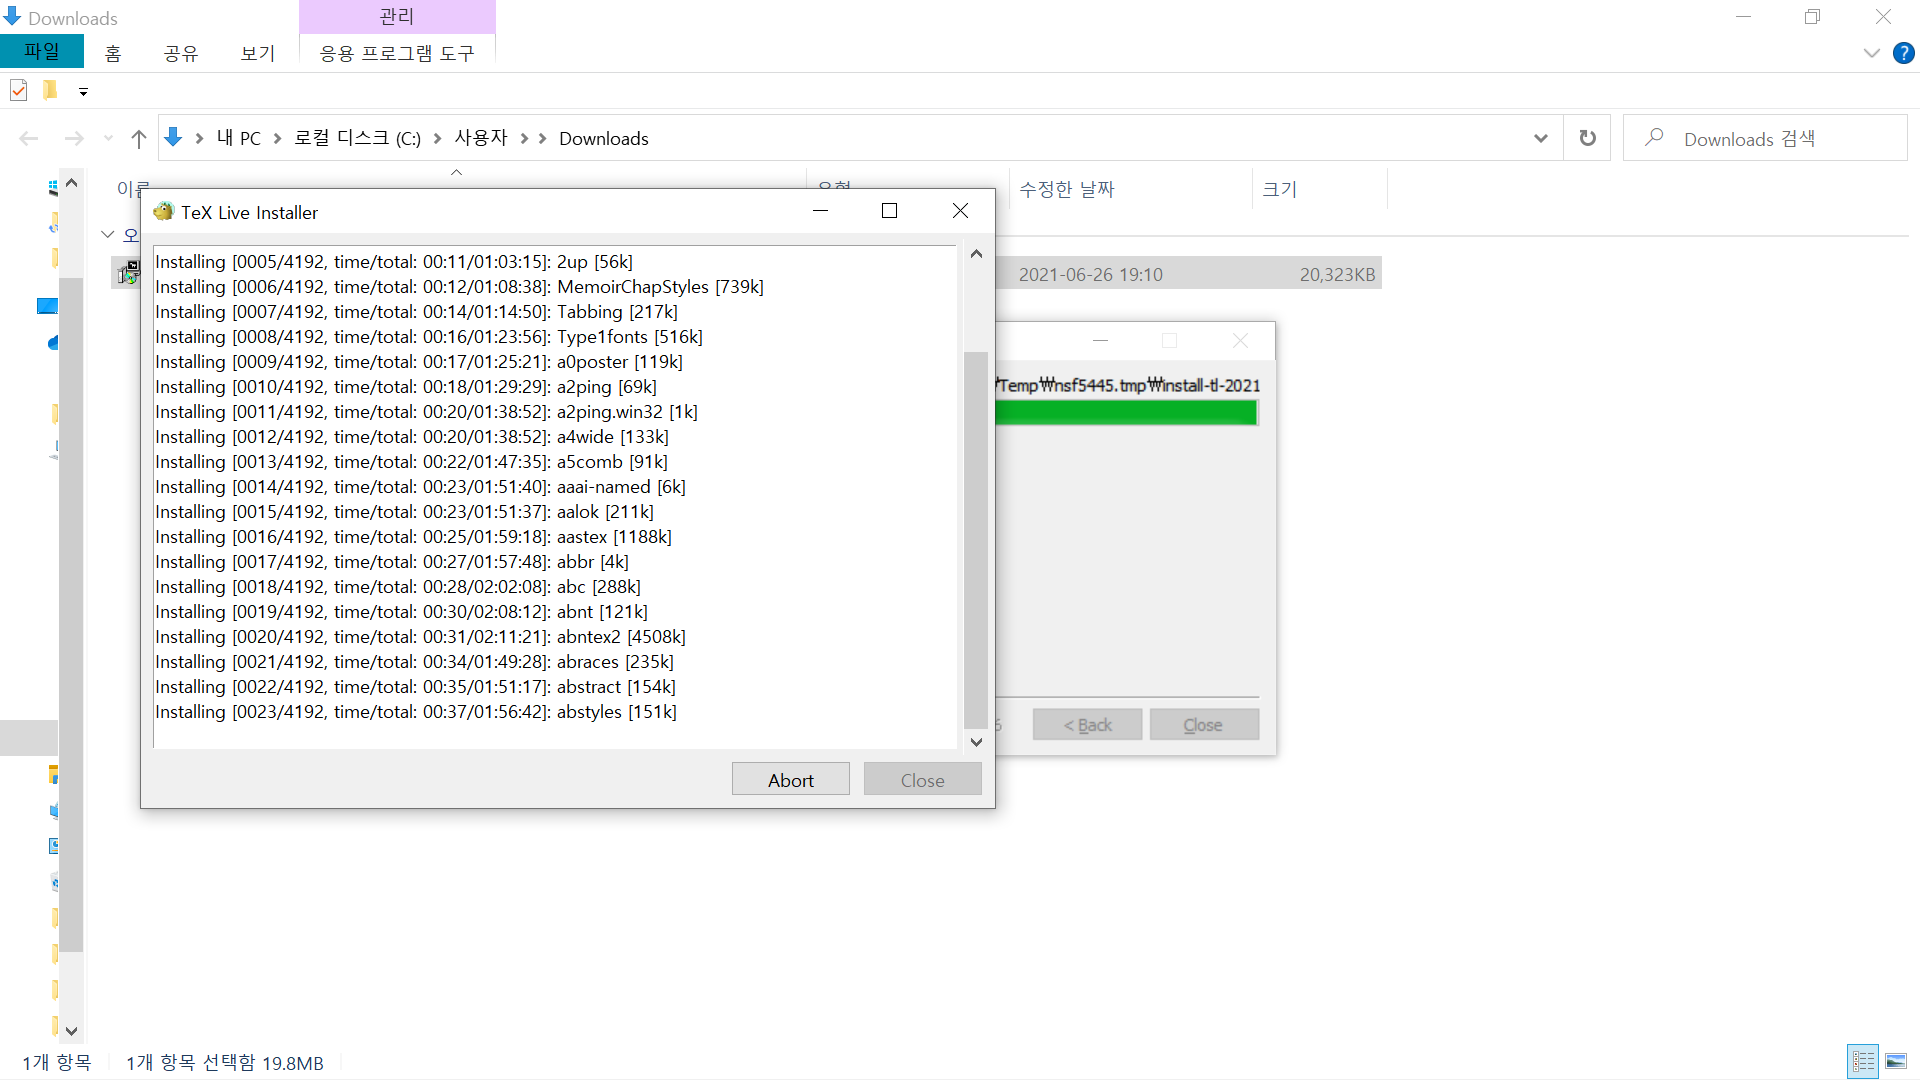
\includegraphics[width=.7\textwidth]{img/5/texlive_install.png}
\caption{Texlive를 설치할 때, 가장 오래 보게 될 장면}
\label{texlive:install}
\end{figure}

\begin{enumerate}
\item 한국 \TeX 사용자 협회 누리집(http://www.ktug.org/)에 접속한다.
\item 실행파일 \href{http://mirror.navercorp.com/CTAN/systems/texlive/tlnet/install-tl-windows.exe}{install-tl-windows.exe}\footnote{주소는 다음과 같다. http://mirror.navercorp.com/CTAN/systems/texlive/tlnet/install-tl-windows.exe}을 다운로드한다. (약 20MB)
\item 실행한다.
\item 어떤 창이 뜨면 `Install'을 누른다.
\item 새로운 창이 뜨는데, `Install'을 누르면 된다.
\item 콘솔창이 뜰 것이다. 현재 다운로드 되는 패키지 이름, 남은 패키지 수와 시간이 표시된다. 대략 2시간~3시간이 표시될 것이다. 여기 표시되는 시간이 다 되어도 끝난 것이 아니니 인내심을 갖고 기다린다.
\item `close'버튼이 활성화가 되면, 설치가 끝난 것이다.
\end{enumerate}

자세한 내용은 `http://wiki.ktug.org/wiki/wiki.php/설치하기Windows/tlinstall'을 참조하여라.

\subsection{\LaTeX 편집하기}
\begin{figure}[h!]
\centering
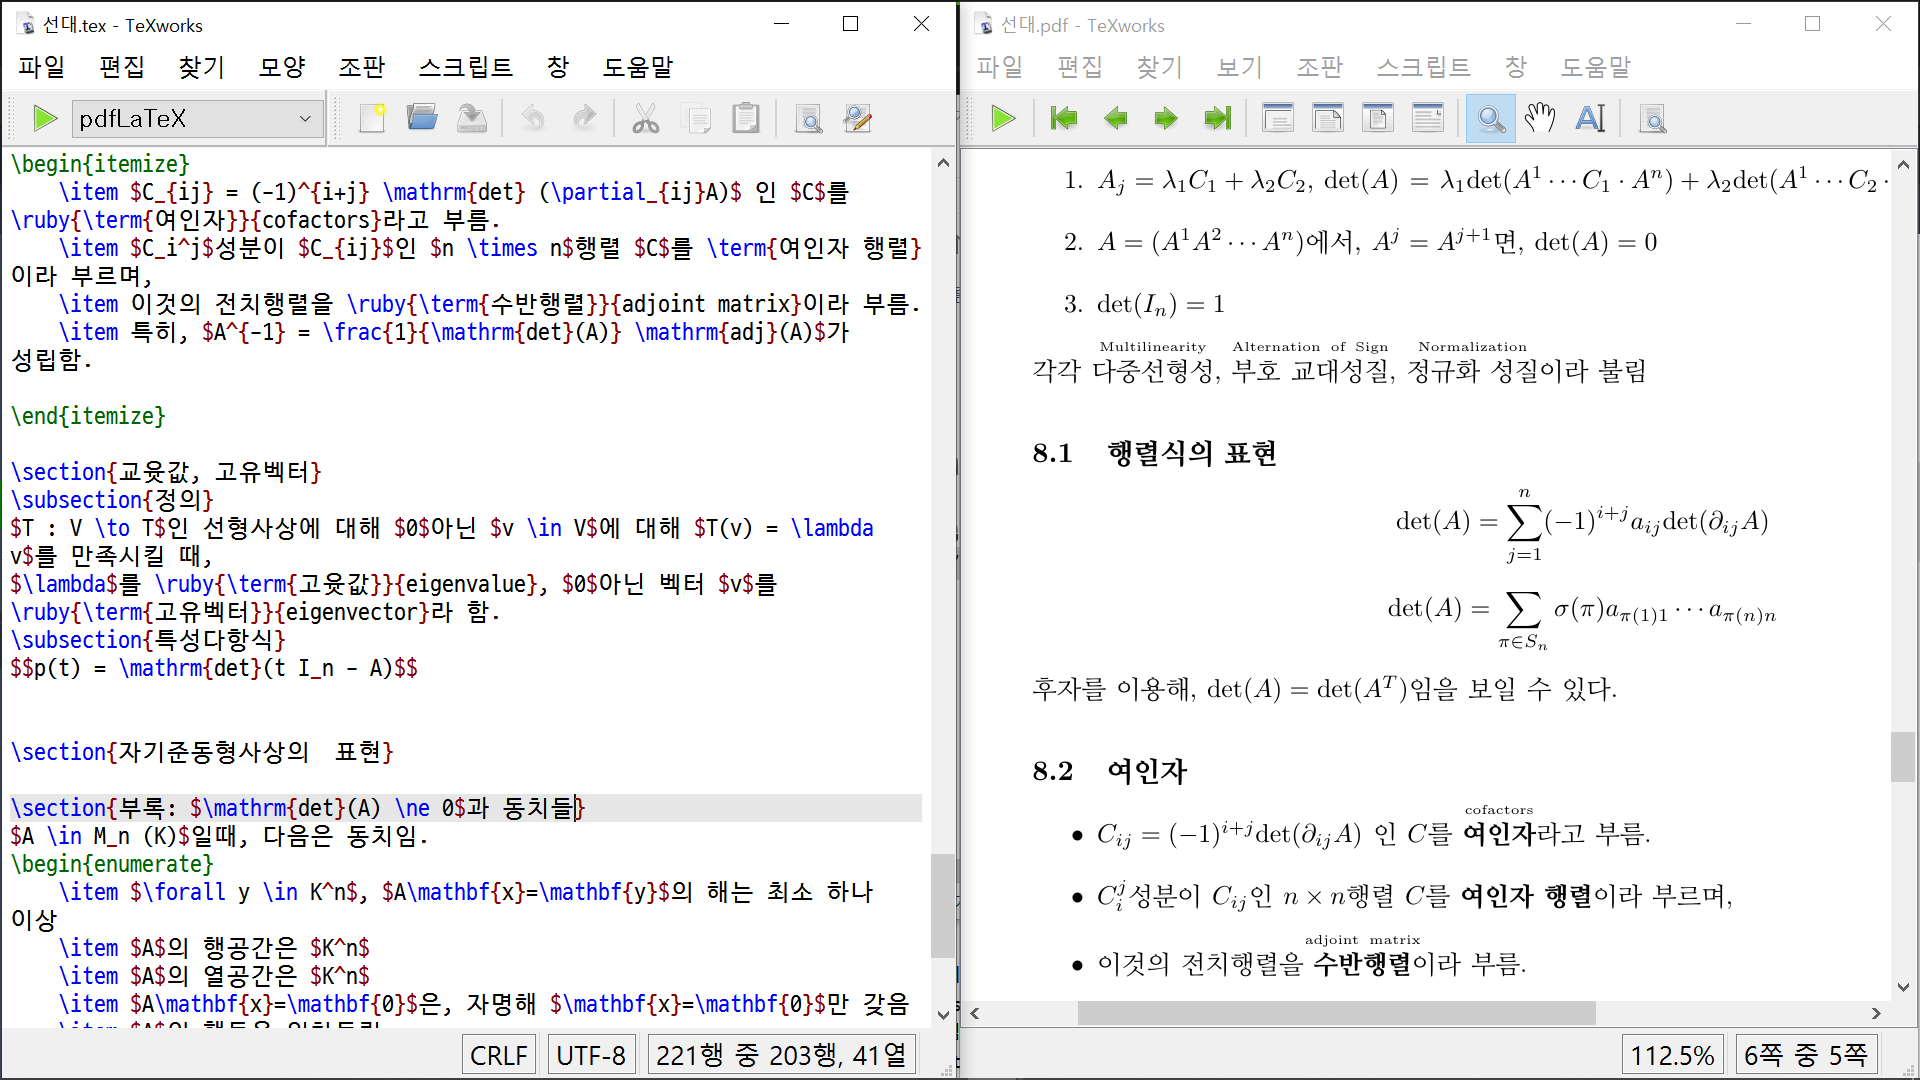
\includegraphics[width=.7\textwidth]{img/5/texlive_edit.png}
\caption{TeXworks 편집 화면}
\label{texlive:exdit}
\end{figure}

\paragraph{TeXworks}
TeXLive를 설치하고 나면 기본적으로 TeXworks라는 에디터가 깔린다. python IDLE와 비슷하게 생긴 외형을 갖고 있다.\footnote{오래된 감성이 느껴진다는 소리다}
하지만, 메뉴의 설명이 한국어로 되어 있다.


에디터를 일단 실행한 뒤, 상단의 'new file'을 눌러 새 파일을 만든다. 그리고 막 편집하면 된다.
저장을 할 때는, 따로 폴더를 하나 만들어서 저장하자. 컴파일을 하게 되면 이것 저것 잡다한 파일들이 생기기 때문이다. 한글 폴더에 저장해도 잘 작동하나, 혹여나 문제가 생길 수 있기 때문에 영어 폴더에 저장하는 것을 추천한다.\footnote{본인은 한글로 된 폴더에 넣고 사용중이나, 아직 아무런 문제점을 느끼지 못했다.}
컴파일러를 선택할 수 있는데, 기본으로 설정된 `pdfLaTeX'도 꽤 쓸만하다.

하지만, 이 기본 에디터를 무작정 쓰다보면 부실하다는 느낌이 든다. 그 이유는 다음과 같았다.
\begin{itemize}
    \item 자동완성 기능이 미흡하다. \verb|\begin{document}|를 치면 \verb|\end{document}|를 자동으로 완성해 주지 않는다. 추천해주는 기능도 없다.
    \item (개인적으로) 디자인이 별로다.
    \item 어느 줄에 오류가 생겼는지 바로 보여주지 않는다.
    \item 컴파일 전에 수식이 문법에 맞게 잘 작성되었는지 확인할 수 없다.
\end{itemize}

부가적인 팁이 있다. 막 설치하고 나면 역슬래시 문자가 ₩로 보인다. 이는 에디터의 글꼴을 역슬래시 문자를 \verb|\|로 표시하는 글꼴로 바꾸면 된다.  필자는 네이버에서 만든 `D2Coding ligature'라는 폰트를 내려받아 사용하고 있다.
`메뉴 > 편집 > 환경설정 > 편집기 > 편집기 기본값'에 있는 빈칸에 원하는 폰트의 이름을 입력하면 된다.

\paragraph{목차 생성}
두 번 저장해야 목차가 생긴다. 컴파일했는데 목차가 만약 생기지 않아 걱정이라면 정상이다. 마음을 가다듬고 다시 한번 더 컴파일하자.

\subsection{고급: \LaTeX을 좀 더 편하게 사용하자}
\LaTeX 관련 에디터를 설치하면 \LaTeX 문서를 쉽고 편리하게 작성할 수 있다. 대표적인 에디터로는 TeXmaker나 Texstudio등이 있다. 본인은 다음과 같은 작성 (?)환경을 구축해서 \LaTeX 문서를 작성하고 있다.

\paragraph{본인 추천: Visual Studio Code 확장기능 이용하기}

\begin{figure}[h!]
\centering
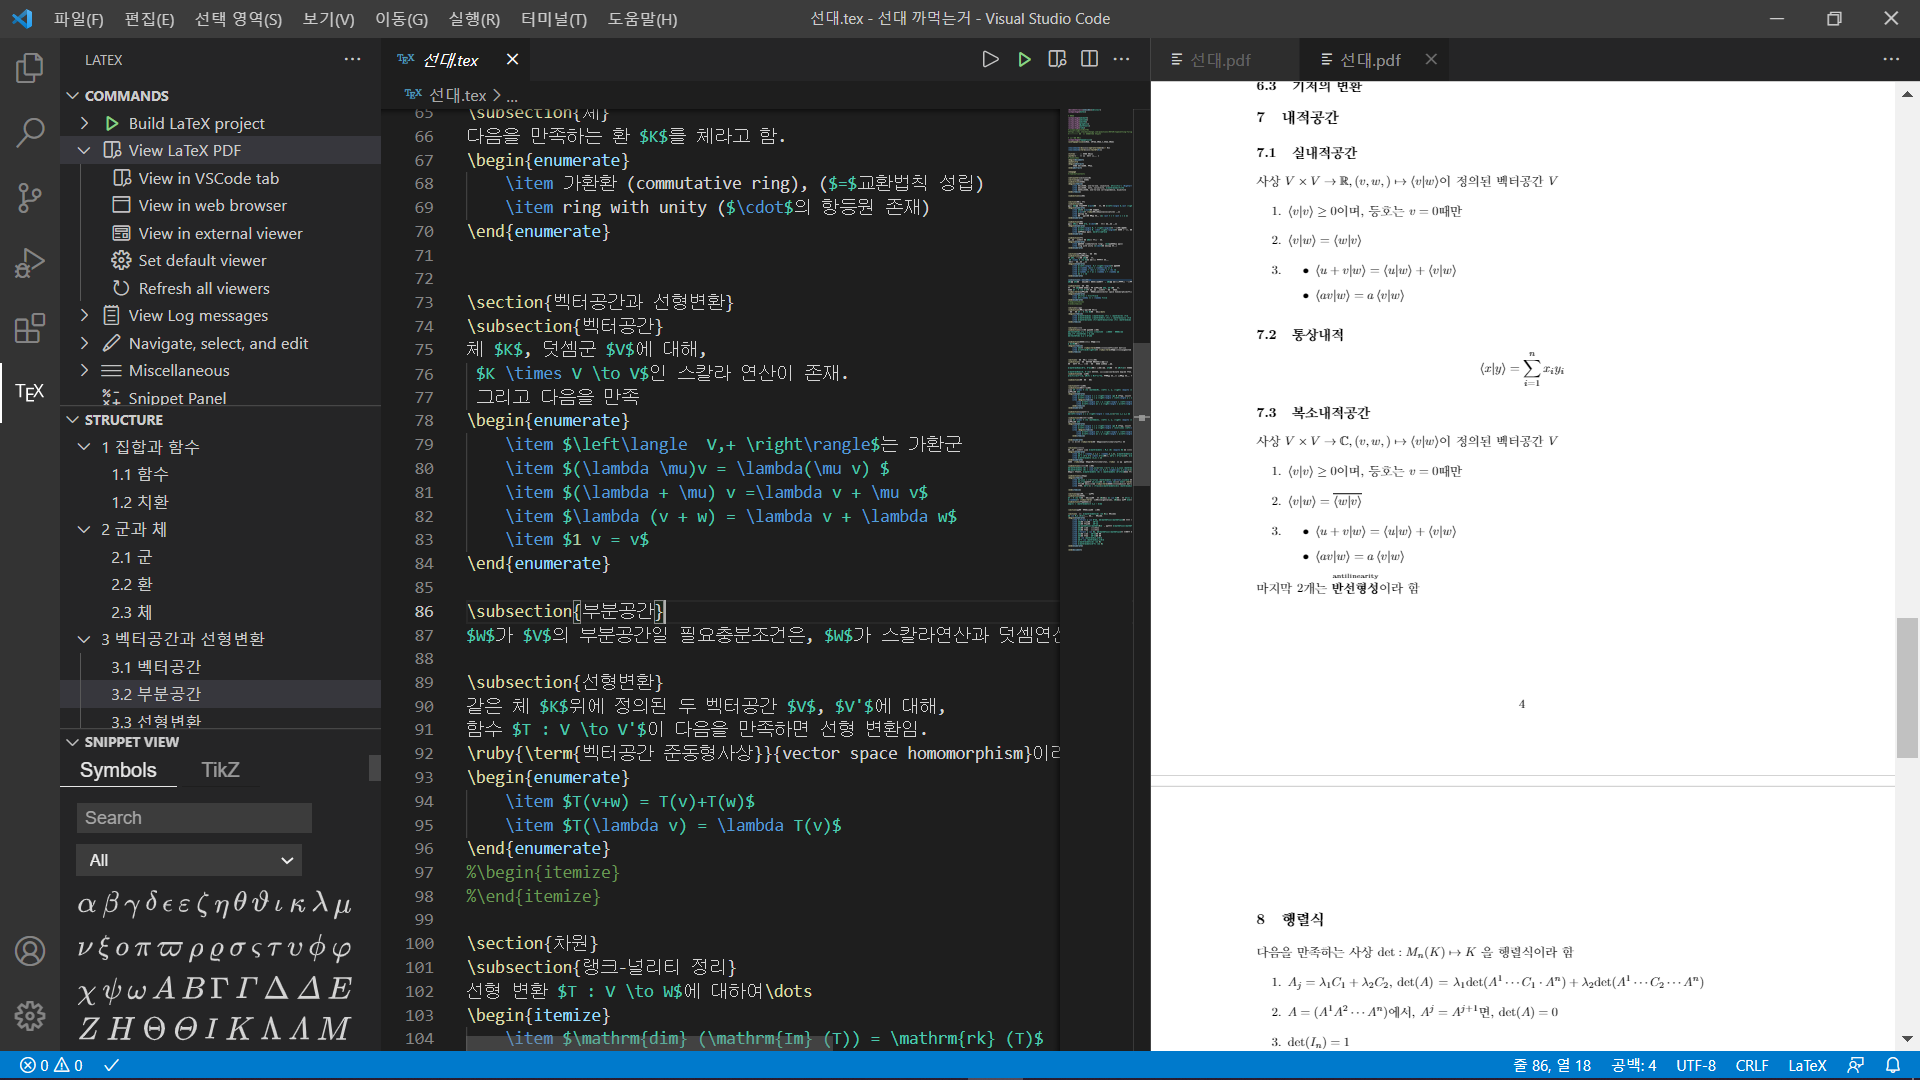
\includegraphics[width=.7\textwidth]{img/5/vs_edit.png}
\caption{Visual Studio Code 편집 화면}
\label{vs:edit}
\end{figure}

평소에 이것저것 코딩을 하는 사람이라면 추천한다. Visual Studio Code\footnote{Visual Studio와는 다른 프로그램이니 주의하자}는 Microsoft사에서 만든 통합 개발 환경이다.\footnote{심지어 오픈소스다!} 쉽게 말하면, 기능 많은 메모장이라고 할 수 있다. Visual Studio Code의 진가는 확장기능이다. Python을 사용하고 싶으면 Python확장 기능을 깔면 되는 것이다.
 \LaTeX Workshop이라는 확장기능을 깔았다.
자동완성 기능, 오류를 코드상에 표시해 주는 기능, 컴파일 전 수식 미리보기 기능 등 효율적이게 하는 기능 등 다양한 기능을 활용할 수 있다.
맞춤법 검사는, 다른 확장 프로그램을 설치해야 한다.



\section{에필로그}
이렇게 해서 어떻게 \LaTeX을 사용할 수 있는지를 살펴 보았다. 이를 통해 여러분도 쉽게 \LaTeX을 이용하게 되었으면 좋겠다. \LaTeX의 드넓은 바다를 자유롭게 헤엄치기를 바란다. 이상.

%\bibliographystyle{plain}
%\bibliography{references}
\end{document}
